\chapter*{ВВЕДЕНИЕ}
\addcontentsline{toc}{chapter}{ВВЕДЕНИЕ}

Системы охранного видеонаблюдения работают в условиях постоянного роста числа камер и объема видеоданных. Ручной мониторинг при такой нагрузке приводит к пропускам событий и увеличению времени реакции. Поэтому основная практическая задача заключается в переходе к автоматическому анализу видеопотоков в режиме, близком к реальному времени.

В отчете рассматривается магистерская работа по теме «Платформы видеоаналитики реального времени для мониторинга и событийного анализа в системах охранного видеонаблюдения». В рамках работы разработана и апробирована платформа, которая выполняет обнаружение объектов, сопровождение во времени, событийную интерпретацию и надежную доставку сведений о событиях внешним потребителям.

Актуальность определяется необходимостью одновременно решать две группы задач: алгоритмические (обнаружение и сопровождение объектов) и инженерные (устойчивый интеграционный контур, безопасность, наблюдаемость) \cite{redmon2016yolo,wojke2017deepsort,transactional_outbox}.

Цель работы состоит в разработке и экспериментальной проверке на исследовательско-экспериментальном стенде платформы видеоаналитики реального времени для мониторинга охраняемых зон и событийного анализа, обеспечивающей обнаружение и сопровождение объектов, формирование интерпретируемых событий и надежную доставку сведений о событиях внешним потребителям.

Для достижения цели необходимо решить следующие задачи:
\begin{enumerate}
    \item проанализировать предметную область охранного видеонаблюдения, существующие подходы к построению платформ видеоаналитики и сформировать функциональные и нефункциональные требования к разрабатываемому решению;
    \item обосновать выбор методов обнаружения объектов, сопровождения объектов и правилового событийного анализа для целевых сценариев видеонаблюдения, включая демонстрационный сценарий обнаружения беспилотных летательных аппаратов;
    \item разработать модель, архитектуру и алгоритмический конвейер платформы, объединяющие прием видеопотока, обнаружение, сопровождение, формирование событий и асинхронную доставку сведений о событиях внешним потребителям;
    \item реализовать программную платформу с компонентами управления, аналитической обработки, интеграционной доставки, разграничения доступа, наблюдаемости и воспроизводимого развертывания;
    \item провести стендовую апробацию платформы по интеграционным, отказным, ролевым и демонстрационным видеосценариям с фиксацией границ доказанности полученных результатов;
    \item определить ограничения текущей реализации, условия ее применимости и направления дальнейшего развития для перехода от исследовательско-экспериментального стенда к промышленному применению.
\end{enumerate}

Объект исследования - процессы автоматизированного мониторинга видеопотоков в системах охранного видеонаблюдения. Предмет исследования - методы, модели и архитектурные решения платформ видеоаналитики реального времени, обеспечивающие обнаружение и сопровождение объектов, формирование событий и надежную доставку сведений о событиях при ограничениях по задержке обработки, отказоустойчивости и безопасности доступа.

\chapter{ПОСТАНОВКА ЗАДАЧИ}
\label{ch:short_problem}

\section{Проблема предметной области}

В охранном видеонаблюдении полезным результатом является не детекция как таковая, а своевременно сформированный факт события. Для этого система должна выполнять четыре связанные функции:
\begin{enumerate}
    \item принимать видеопоток и поддерживать стабильную обработку кадров;
    \item обнаруживать и классифицировать объекты;
    \item сопровождать их во времени с сохранением идентичности;
    \item интерпретировать траектории в терминах событий и надежно доставлять сведения о событиях.
\end{enumerate}

Пусть для камеры \(i\) поток кадров обозначен как \(\{x_t^i\}\). Тогда целевой конвейер задается последовательностью преобразований:
\begin{equation}
\mathcal{V} \rightarrow \mathcal{D} \rightarrow \mathcal{T} \rightarrow \mathcal{E} \rightarrow \texttt{event\_outbox},
\end{equation}
\noindent\hspace*{\parindent}где \(\mathcal{D}\) \textemdash\ детекции;
\par\noindent\hspace*{\parindent}\(\mathcal{T}\) \textemdash\ треки;
\par\noindent\hspace*{\parindent}\(\mathcal{E}\) \textemdash\ события.

Графически сквозной маршрут показан на рисунке~\ref{fig:short_pipeline}. Каждый узел представляет дискретный этап преобразования данных, переход между этапами реализован через явный программный контракт.

\begin{figure}[H]
\centering
\begin{tikzpicture}[
    node distance=6mm and 7mm,
    every node/.style={font=\small},
    stage/.style={
        draw=cBorder, line width=0.4pt, rounded corners=2pt,
        fill=cBox, text=cText,
        minimum width=22mm, minimum height=11mm,
        align=center, inner sep=3pt
    },
    sink/.style={stage, fill=cBoxAcc},
    src/.style={stage, fill=cBoxAlt},
    arr/.style={-{Stealth[length=2.2mm]}, draw=cArrow, line width=0.5pt}
]
\node[src] (cam) {RTSP\\поток};
\node[stage, right=of cam] (det) {Детектор\\YOLO};
\node[stage, right=of det] (trk) {Сопровождение\\DeepSORT};
\node[stage, right=of trk] (rule) {Правиловой\\движок};
\node[stage, below=10mm of rule] (out) {\texttt{event\_outbox}\\(PostgreSQL)};
\node[stage, left=of out] (br) {Брокер\\RabbitMQ};
\node[sink, left=of br] (wh) {HTTP-\\получатель};
\draw[arr] (cam) -- (det);
\draw[arr] (det) -- node[above,font=\tiny]{bbox} (trk);
\draw[arr] (trk) -- node[above,font=\tiny]{траект.} (rule);
\draw[arr] (rule) -- node[right,font=\tiny]{событие} (out);
\draw[arr] (out) -- node[above,font=\tiny]{публ.} (br);
\draw[arr] (br) -- node[above,font=\tiny]{дост.} (wh);
\end{tikzpicture}
\caption{Сквозной конвейер обработки видео и доставки событий}
\label{fig:short_pipeline}
\end{figure}

\section{Ключевые требования}

Требования зафиксированы в связке «требование - проверка».

\begin{table}[H]
\caption{Ключевые требования к платформе}
\label{tab:short_requirements}
\begin{tabularx}{\textwidth}{>{\raggedright\arraybackslash}p{0.35\textwidth}X}
\toprule
Требование & Практический критерий \\
\midrule
Работа в режиме реального времени & Ограниченный p95 \texttt{object->event}, отсутствие неограниченного роста очередей \\
Надежность интеграции & Сохранение событий в таблице исходящих сообщений при отказах, успешная обработка накопленной очереди после восстановления \\
Интерпретируемость событий & Явное правило формирования (\texttt{zone\_enter}, \texttt{line\_cross}, \texttt{dwell\_time}) и трассируемый \texttt{dedup\_key} \\
Безопасность доступа & Корректный сценарий JWT-аутентификации, соблюдение RBAC-ограничений для ролей \texttt{admin/operator/viewer} \\
Воспроизводимость эксплуатации & Единый compose-стенд, наблюдаемость через \texttt{/health} и \texttt{/metrics} \\
\bottomrule
\end{tabularx}
\end{table}

\section{Принятые ограничения}

Чтобы получить измеримый и воспроизводимый результат в магистерском проекте, осознанно приняты ограничения:
\begin{itemize}
    \item базовый охранный профиль ориентирован на классы \texttt{person} и \texttt{vehicle}; БПЛА вынесены в отдельный демонстрационный профиль с классами \texttt{bird} и \texttt{drone};
    \item камерно-изолированное сопровождение без межкамерной повторной идентификации (ReID);
    \item односерверный контур развертывания;
    \item ограниченный, но интерпретируемый набор событийных правил.
\end{itemize}

\section{Цель и ожидаемый результат}

Цель работы состоит в разработке и экспериментальной проверке на исследовательско-экспериментальном стенде платформы видеоаналитики реального времени для мониторинга охраняемых зон и событийного анализа, обеспечивающей обнаружение и сопровождение объектов, формирование интерпретируемых событий и надежную доставку сведений о событиях внешним потребителям.

Ожидаемый результат - воспроизводимый исследовательско-экспериментальный стенд платформы, в котором подтверждены:
\begin{enumerate}
    \item корректность интеграционной доставки синтетически зафиксированных событий \texttt{zone\_enter}, \texttt{line\_cross} и \texttt{dwell\_time};
    \item связность демонстрационного видеоконтура БПЛА от обученной модели до траекторий, событий и операторского интерфейса;
    \item устойчивость контуров доставки при инфраструктурных сбоях;
    \item работоспособность ролевой модели доступа;
    \item наблюдаемость состояния платформы по ключевым метрикам.
\end{enumerate}

\chapter{АРХИТЕКТУРА И АЛГОРИТМИЧЕСКИЙ ПОДХОД}
\label{ch:short_arch}

\section{Логика архитектуры}

Архитектура построена как набор специализированных сервисов с четким разделением ответственности:
\begin{itemize}
    \item \texttt{api} - управление конфигурацией, доступом и журналом событий;
    \item \texttt{analytics-worker} - обработка видеопотоков и генерация событий;
    \item \texttt{integration-worker} - доставка событий через брокер и HTTP-получатель;
    \item \texttt{ui} - операторские сценарии;
    \item инфраструктура: PostgreSQL, RabbitMQ, Prometheus, Grafana.
\end{itemize}

Контекстный уровень C4 (рисунок~\ref{fig:short_c4_context}) отражает положение платформы относительно внешних участников: оператор и администратор работают через пользовательский интерфейс и API, IP-камеры подают RTSP-поток, а внешние корпоративные системы получают события через HTTP-получатель.

\begin{figure}[H]
\centering
\begin{tikzpicture}[
    every node/.style={font=\small},
    actor/.style={
        draw=cBorder, line width=0.4pt, rounded corners=2pt,
        fill=cBoxAlt, text=cText,
        minimum width=24mm, minimum height=12mm, align=center, inner sep=3pt
    },
    sys/.style={
        draw=cBorder, line width=0.6pt, rounded corners=3pt,
        fill=cBoxAcc, text=cText,
        minimum width=46mm, minimum height=20mm, align=center, inner sep=4pt
    },
    ext/.style={
        draw=cBorder, line width=0.4pt, rounded corners=2pt,
        fill=cBox, text=cText,
        minimum width=24mm, minimum height=12mm, align=center, inner sep=3pt
    },
    arr/.style={-{Stealth[length=2.2mm]}, draw=cArrow, line width=0.5pt}
]
\node[actor] (op)  at (-5.5,1.4) {Оператор};
\node[actor] (adm) at (-5.5,-1.4) {Администратор};
\node[sys]   (sys) at (0,0) {\textbf{Платформа}\\\textbf{видеоаналитики}\\\footnotesize реального времени};
\node[ext]   (cam) at (5.5,1.4) {IP-камеры\\\footnotesize RTSP};
\node[ext]   (ext) at (5.5,-1.4) {Внешние\\системы\\\footnotesize HTTP-получатель};
\draw[arr] (op)  -- node[above,font=\scriptsize]{интерфейс} (sys);
\draw[arr] (adm) -- node[below,font=\scriptsize]{API} (sys);
\draw[arr] (cam) -- node[above,font=\scriptsize]{видео} (sys);
\draw[arr] (sys) -- node[below,font=\scriptsize]{события} (ext);
\end{tikzpicture}
\caption{C4: контекстный уровень платформы и внешние участники}
\label{fig:short_c4_context}
\end{figure}

Уровень контейнеров (рисунок~\ref{fig:short_c4_container}) детализирует внутреннюю композицию: контур управления (API, пользовательский интерфейс, БД), контур обработки данных (\texttt{analytics-worker}, \texttt{integration-worker}, RabbitMQ) и инфраструктура наблюдаемости.

\begin{figure}[H]
\centering
\begin{tikzpicture}[
    scale=0.82,
    transform shape,
    every node/.style={font=\small},
    cont/.style={
        draw=cBorder, line width=0.4pt, rounded corners=2pt,
        fill=cBox, text=cText,
        minimum width=28mm, minimum height=11mm, align=center, inner sep=3pt
    },
    db/.style={cont, fill=cBoxAcc},
    bus/.style={cont, fill=cBoxAlt},
    obs/.style={cont, fill=cBoxAcc},
    actor/.style={
        draw=cBorder, line width=0.4pt, rounded corners=2pt,
        fill=cBoxAlt, text=cText,
        minimum width=20mm, minimum height=10mm, align=center, inner sep=3pt
    },
    arr/.style={-{Stealth[length=2.2mm]}, draw=cArrow, line width=0.5pt},
    arrd/.style={-{Stealth[length=2.2mm]}, draw=cArrow, line width=0.4pt, dashed}
]
\node[actor] (cam) at (-6.5,2.2) {IP-камеры};
\node[actor] (op)  at (-6.5,0.4) {Оператор};
\node[actor] (ext) at (6.6,0.4) {Внешние\\системы};
\node[cont] (aw)  at (-3,2.2) {analytics-worker\\\footnotesize детекция, траектории, правила};
\node[cont] (ui)  at (-3,0.4) {ui\\\footnotesize React + nginx};
\node[cont] (api) at ( 0.5,0.4) {api\\\footnotesize FastAPI, JWT, RBAC};
\node[db]   (pg)  at ( 0.5,-1.6) {PostgreSQL\\\footnotesize events, event\_outbox};
\node[bus]  (mq)  at ( 4,0.4) {RabbitMQ};
\node[cont] (iw)  at ( 4,-1.6) {integration-worker\\\footnotesize публикация + повторы + очередь недоставл.};
\node[obs]  (prom) at (-3,-1.6) {Prometheus\\\footnotesize + Grafana};
\draw[arr] (cam) -- node[above,font=\scriptsize]{RTSP} (aw);
\draw[arr] (op)  -- (ui);
\draw[arr] (ui)  -- node[above,font=\scriptsize]{REST} (api);
\draw[arr] (api) -- node[right,font=\scriptsize]{SQL} (pg);
\draw[arr] (aw) -| node[pos=0.25,above,font=\scriptsize]{исходящие} (pg);
\draw[arr] (pg) -- node[above,font=\scriptsize]{опрос} (iw);
\draw[arr] (iw) -- node[right,font=\scriptsize]{публикация} (mq);
\draw[arr] (mq) -- (ext);
\draw[arrd] (aw) -- node[left,font=\scriptsize]{/metrics} (prom);
\draw[arrd] (api) -- (prom);
\draw[arrd] (iw) -- (prom);
\end{tikzpicture}
\caption{C4: контейнерный уровень и композиция сервисов платформы}
\label{fig:short_c4_container}
\end{figure}

\section{Алгоритмический конвейер}

В основе аналитического слоя - связка детектор + модуль сопровождения + правиловой движок.

\subsection{Детекция}

В качестве базового метода выбран одноэтапный детектор семейства YOLO как компромисс между скоростью и точностью в потоковой обработке \cite{redmon2016yolo}. После инференса применяются порог достоверности и подавление дубликатов по IoU.

Пример отклика демонстрационного БПЛА-профиля показан на рисунке~\ref{fig:short_detection_demo}: для классов \texttt{bird} и \texttt{drone} формируются прямоугольные рамки с оценкой достоверности, которые далее передаются в модуль сопровождения.

\begin{figure}[H]
\centering
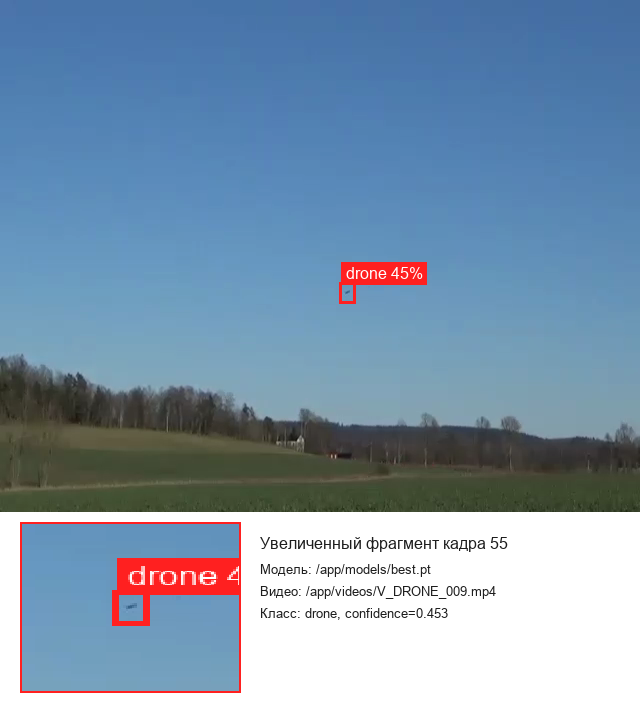
\includegraphics[width=0.78\textwidth]{drone_demo_detection.png}
\caption{Пример отклика детектора в демонстрационном БПЛА-сценарии}
\label{fig:short_detection_demo}
\end{figure}

\subsection{Сопровождение}

Для устойчивого сохранения идентичности используется подход сопровождения по результатам обнаружения, реализованный в логике DeepSORT: он сочетает кинематический прогноз и признаки внешнего вида \cite{wojke2017deepsort}. Это снижает число переключений идентификаторов при частичных перекрытиях и временных пропусках детекций.

\subsection{Событийный анализ}

Событие формируется правилом, заданным как пространственно-временной предикат над траекторией:
\begin{equation}
e_r = P_r(\tau_j, \mathcal{Z}, t),
\end{equation}
\where
\whereitemlast{\(P_r\)}{предикат правила одного из типов: \texttt{zone\_enter}, \texttt{line\_cross}, \texttt{dwell\_time}}

Реализация правил локализована в классе \texttt{RuleEngine}: для каждого трека хранится последняя позиция и время входа в зону, а проверка выполняется по геометрическим предикатам. Листинг~\ref{lst:short_rule_engine} приведен из файла \texttt{services/analytics-worker/app/rule\_engine.py}.

\begin{lstlisting}[language=Python,caption={Фрагмент правил \texttt{line\_cross} и \texttt{dwell\_time}},label={lst:short_rule_engine}]
if rule_type == "line_cross":
    line_points = (params.get("line") or [])
    if len(line_points) == 2 and st.last_point is not None:
        p1 = (float(line_points[0][0]), float(line_points[0][1]))
        p2 = (float(line_points[1][0]), float(line_points[1][1]))
        line_key = f"line_cross:{rule['rule_id']}:{track_id}"
        if segments_intersect(st.last_point, current_point, p1, p2) \
                and line_key not in st.fired_keys:
            st.fired_keys.add(line_key)
            dedup = f"{self.camera_id}:{rule['rule_id']}:{track_id}:line_cross"
            generated.append(self._build_event(
                track=track, rule=rule,
                event_type="line_cross",
                dedup_key=dedup, zone_id=zone_id,
            ))

if rule_type == "dwell_time" and zone:
    threshold = int(params.get("seconds", 5))
    polygon = (zone.get("geometry") or {}).get("points", [])
    inside = point_in_polygon(current_point, polygon)
    if inside:
        start_ts = st.zone_entered_at.setdefault(zone_id, ts)
        dwell_key = f"{rule['rule_id']}:{zone_id}:{track_id}:{threshold}"
        if (ts - start_ts).total_seconds() >= threshold \
                and dwell_key not in st.fired_keys:
            st.fired_keys.add(dwell_key)
            ...
\end{lstlisting}

Здесь \texttt{fired\_keys} обеспечивает идемпотентность срабатывания: повторный вход траектории в ту же зону в рамках одного активного эпизода не приводит к дублированию события. Поле \texttt{dedup\_key} включает идентификаторы камеры, правила и траектории, что позволяет внешнему потребителю безопасно повторно обрабатывать сообщения.

\section{Надежная доставка событий}

Ключевое инженерное решение - транзакционная таблица исходящих сообщений \cite{transactional_outbox,rabbitmq_docs}. Событие и запись исходящего сообщения фиксируются в одной транзакции БД, после чего публикация в брокер выполняется асинхронно:
\begin{equation}
\operatorname{commit}(\text{событие}, \text{исходящее сообщение}) \Rightarrow \text{событие не теряется}.
\end{equation}
При временной недоступности брокера событие остается в таблице исходящих сообщений и публикуется после восстановления внешнего контура.
Для интеграционного слоя используется политика повторов с ограниченной задержкой между попытками и маршрутизацией в очередь недоставленных сообщений после исчерпания попыток. Это дает контролируемое поведение в отказных режимах и прозрачную диагностику.

Жизненный цикл сообщения по контурам ответственности показан на рисунке~\ref{fig:short_seq_outbox}: фиксация события и записи исходящего сообщения выполняется в одной транзакции, а доставка продолжается асинхронно даже при кратковременной недоступности RabbitMQ или HTTP-получателя.

\begin{figure}[H]
\centering
\begin{tikzpicture}[
    every node/.style={font=\footnotesize},
    actor/.style={
        draw=cBorder, line width=0.4pt, rounded corners=2pt,
        fill=cBoxAlt, text=cText,
        minimum width=22mm, minimum height=8mm, align=center
    },
    msg/.style={-{Stealth[length=2mm]}, draw=cArrow, line width=0.4pt},
    note/.style={font=\scriptsize\itshape, text=cText, align=center}
]
\node[actor] (aw)  at (0,0)   {analytics-worker};
\node[actor] (db)  at (3.5,0) {PostgreSQL};
\node[actor] (iw)  at (7,0)   {integration-worker};
\node[actor] (mq)  at (10.5,0){RabbitMQ};
\node[actor] (wh)  at (14,0)  {HTTP-\\получатель};
\foreach \n in {aw,db,iw,mq,wh} {\draw[gray,dashed,line width=0.3pt] (\n.south) -- ++(0,-7);}

\draw[msg] ($(aw.south)+(0,-0.5)$) -- node[above,font=\scriptsize]{INSERT events + event\_outbox (TX)} ($(db.south)+(0,-0.5)$);
\node[note] at (1.7,-1.1) {фиксация};

\draw[msg] ($(iw.south)+(0,-1.6)$) -- node[above,font=\scriptsize]{SELECT pending} ($(db.south)+(0,-1.6)$);
\draw[msg] ($(db.south)+(0,-2.1)$) -- node[above,font=\scriptsize]{записи} ($(iw.south)+(0,-2.1)$);

\draw[msg] ($(iw.south)+(0,-2.8)$) -- node[above,font=\scriptsize]{publish(event)} ($(mq.south)+(0,-2.8)$);
\node[note] at (8.7,-3.3) {опубликовано};

\draw[msg] ($(mq.south)+(0,-4)$) -- node[above,font=\scriptsize]{POST /webhook} ($(wh.south)+(0,-4)$);
\draw[msg] ($(wh.south)+(0,-4.5)$) -- node[above,font=\scriptsize]{2xx} ($(mq.south)+(0,-4.5)$);

\draw[msg] ($(iw.south)+(0,-5.4)$) -- node[above,font=\scriptsize]{UPDATE outbox set published\_at} ($(db.south)+(0,-5.4)$);

\draw[msg,dashed] ($(wh.south)+(0,-6.2)$) -- node[above,font=\scriptsize]{ошибка $\rightarrow$ повтор, затем очередь недост.} ($(mq.south)+(0,-6.2)$);
\end{tikzpicture}
\caption{Диаграмма последовательности доставки события через таблицу исходящих сообщений}
\label{fig:short_seq_outbox}
\end{figure}

Реализация цикла публикации в \texttt{integration-worker} выделяет три явные позиции отказа: соединение с брокером, публикацию сообщения и подтверждение записи исходящего сообщения. На каждом из них предусмотрена реакция, отделяющая повторяемые ошибки от конечных. Листинг~\ref{lst:short_publisher_loop} приведен из \texttt{services/integration-worker/app/main.py}.

\begin{lstlisting}[language=Python,caption={Цикл публикации исходящих сообщений с ограниченными повторами},label={lst:short_publisher_loop}]
candidates = fetch_publish_candidates(limit=100)
for row in candidates:
    outbox_id = row["outbox_id"]
    retry_count = int(row.get("retry_count", 0))
    payload = row["payload"]
    event_type = payload.get("event_type", "unknown")
    try:
        broker.publish_event(payload, event_type)
        mark_published(outbox_id)
        PUBLISH_SUCCESS.inc()
    except Exception as exc:
        retry_count += 1
        terminal = retry_count >= settings.max_retry
        mark_retry(outbox_id, retry_count, terminal=terminal)
        PUBLISH_ERROR.inc()
        if not terminal:
            OUTBOX_RETRIES.inc()
        # ошибка брокера: переподключаемся и продолжаем со следующего пакета
        reconnect_required = True
        break
\end{lstlisting}

Логика обработчика сообщения (доставка HTTP-получателю) дополняется экспоненциальной задержкой между повторами и переходом в очередь недоставленных сообщений после исчерпания попыток (листинг~\ref{lst:short_consumer_dlq}).

\begin{lstlisting}[language=Python,caption={Доставка HTTP-получателю с повтором и переходом в очередь недоставленных сообщений},label={lst:short_consumer_dlq}]
success, error_text = _deliver_webhook(payload)
if success:
    WEBHOOK_SUCCESS.inc()
    log_delivery_attempt(event_id, consumer_name, "success", None)
    channel.basic_ack(delivery_tag=method.delivery_tag)
    return

WEBHOOK_FAILURE.inc()
log_delivery_attempt(event_id, consumer_name, "failed", error_text)
next_attempt = attempt + 1
if next_attempt >= settings.max_retry:
    broker.publish_dlq(payload, reason=error_text or "max_retries")
    DLQ_PUBLISH.inc()
    channel.basic_ack(delivery_tag=method.delivery_tag)
    return

time.sleep(min(30, 2 ** next_attempt))  # экспоненциальная задержка
broker.publish_event(payload, payload.get("event_type", "unknown"),
                     headers={"delivery_attempt": next_attempt})
\end{lstlisting}

\section{Наблюдаемость и управление качеством}

Платформа проектировалась как наблюдаемая система. В каждом сервисе реализованы:
\begin{itemize}
    \item \texttt{/health/live}, \texttt{/health/ready};
    \item \texttt{/metrics} для Prometheus;
    \item журналирование действий и ошибок по сервисным сценариям.
\end{itemize}

Ключевые эксплуатационные метрики:
\begin{enumerate}
    \item p95 задержка \texttt{object->event};
    \item доля отброшенных кадров;
    \item размер накопленной очереди исходящих сообщений и число повторов;
    \item число сообщений в очереди недоставленных;
    \item успешность доставки HTTP-получателю.
\end{enumerate}

\section{Архитектурные драйверы и границы системы}

Архитектура второй итерации отчета уточнена через набор архитектурных драйверов, которые напрямую влияют на структуру компонентов:
\begin{itemize}
    \item актуальность события важнее обработки каждого кадра без исключения;
    \item отказ внешней интеграции не должен блокировать аналитический контур;
    \item замена детектора или модуля сопровождения должна быть локальным изменением;
    \item эксплуатационная диагностика должна выполняться без доступа к исходному коду;
    \item конфигурация камер и правил должна изменяться без остановки всей платформы.
\end{itemize}

По этой причине система разделена на два функциональных слоя:
\begin{itemize}
    \item контур управления - API управления, конфигурация, аудит, ролевой доступ;
    \item контур обработки данных - захват потока, инференс, сопровождение объектов, формирование и доставка событий.
\end{itemize}

Практический эффект такого разделения состоит в том, что при проблемах в контуре управления допустима продолженная обработка видео по уже загруженным правилам, а при временной перегрузке контура обработки данных административные функции остаются доступными.

\section{Поток данных и контракты взаимодействия}

Сквозной маршрут в эксплуатационном режиме фиксируется как последовательность этапов:
\begin{enumerate}
    \item прием RTSP-потока и декодирование;
    \item нормализация таймштампов и отбор актуального кадра;
    \item инференс детектора и фильтрация дубликатов;
    \item обновление состояния траекторий по камере;
    \item применение правил к траекториям;
    \item транзакционная фиксация \texttt{events} и \texttt{event\_outbox};
    \item асинхронная публикация в брокер;
    \item доставка во внешний HTTP-получатель или API.
\end{enumerate}

Для устранения неоднозначностей в интеграции закреплен минимальный контракт события (таблица~\ref{tab:short_event_contract}).

\begin{table}[H]
\caption{Минимальный контракт доменного события}
\label{tab:short_event_contract}
\begin{tabularx}{\textwidth}{>{\raggedright\arraybackslash}p{0.28\textwidth}p{0.2\textwidth}X}
\toprule
Поле & Тип & Назначение \\
\midrule
\texttt{event\_id} & UUID & Уникальный идентификатор события \\
\texttt{event\_type} & string & Тип события: \texttt{zone\_enter}, \texttt{line\_cross}, \texttt{dwell\_time} \\
\texttt{camera\_id} & UUID/string & Камера-источник события \\
\texttt{track\_id} & integer & Идентификатор траектории внутри камеры \\
\texttt{event\_time} & timestamp & Момент выполнения правила \\
\texttt{rule\_id} & UUID/string & Правило, сгенерировавшее событие \\
\texttt{dedup\_key} & string & Ключ дедупликации при повторной доставке \\
\texttt{payload} & JSON & Расширенные данные: зона, линия, оценка достоверности, bbox \\
\bottomrule
\end{tabularx}
\end{table}

Внутренний API проектируется по принципу явных границ: синхронные HTTP-вызовы используются только для управления и чтения состояния, а доменные события и интеграция выносятся в асинхронный контур.

\section{Модель данных и жизненный цикл события}

Событийная запись проходит набор дискретных состояний:
\begin{enumerate}
    \item \texttt{created} - событие сформировано правилом;
    \item \texttt{persisted} - запись сохранена в \texttt{events} и \texttt{event\_outbox};
    \item \texttt{published} - сообщение подтверждено брокером;
    \item \texttt{delivered} - внешний получатель подтвердил прием;
    \item \texttt{dead\_letter} - попытки исчерпаны, запись перенаправлена в очередь недоставленных.
\end{enumerate}

ER-диаграмма ключевых таблиц предметной области (рисунок~\ref{fig:short_er}) показывает связи между конфигурацией (камеры, зоны, правила), оперативным состоянием (траектории) и фактологическим слоем (события и исходящие сообщения). Дедупликация событий обеспечивается уникальностью \texttt{dedup\_key} в таблице \texttt{events}, а \texttt{event\_outbox} разделяет фиксацию факта и публикацию сообщения.

\begin{figure}[H]
\centering
\begin{tikzpicture}[
    every node/.style={font=\scriptsize},
    ent/.style={
        draw=cBorder, line width=0.4pt, rounded corners=2pt,
        fill=cBox, text=cText,
        minimum width=34mm, align=left, inner sep=4pt
    },
    ent2/.style={ent, fill=cBoxAcc},
    ent3/.style={ent, fill=cBoxAlt},
    rel/.style={-{Stealth[length=2mm]}, draw=cArrow, line width=0.4pt}
]
\node[ent]  (cam)   at (0,3)    {\textbf{cameras}\\camera\_id PK\\name, rtsp\_url\\status, fps\_target};
\node[ent]  (zone)  at (5.2,4.4){\textbf{zones}\\zone\_id PK\\camera\_id FK\\geometry (JSON)};
\node[ent]  (rule)  at (5.2,1.6){\textbf{rules}\\rule\_id PK\\camera\_id FK\\rule\_type, params};
\node[ent]  (trk)   at (0,-0.4) {\textbf{tracks}\\(track\_id, camera\_id) PK\\object\_class\\last\_bbox, state};
\node[ent2] (ev)    at (5.2,-1) {\textbf{events}\\event\_id PK\\camera\_id, track\_id\\rule\_id FK\\event\_type, severity\\\textbf{dedup\_key UNIQUE}};
\node[ent3] (out)   at (10.5,-1){\textbf{event\_outbox}\\outbox\_id PK\\event\_id FK\\status, retry\_count\\next\_retry\_at};
\node[ent]  (att)   at (10.5,-3.6){\textbf{delivery\_attempts}\\attempt\_id PK\\event\_id, consumer\_name\\status, attempted\_at};
\draw[rel] (cam.east) -- node[above,sloped]{1..N} (zone.west);
\draw[rel] (cam.east) -- node[below,sloped]{1..N} (rule.west);
\draw[rel] (cam.south) -- node[right]{1..N} (trk.north);
\draw[rel] (rule.south) -- node[right]{1..N} (ev.north);
\draw[rel] (ev.east) -- node[above]{1..1} (out.west);
\draw[rel] (ev.south) |- node[pos=0.25,right]{1..N} (att.west);
\end{tikzpicture}
\caption{ER-диаграмма ключевых таблиц предметной области}
\label{fig:short_er}
\end{figure}

Декларация ORM для событий и исходящих сообщений приведена в листинге~\ref{lst:short_models} (фрагмент \texttt{services/api/app/models.py}). Уникальность \texttt{dedup\_key} вынесена на уровень схемы, что исключает повторную вставку даже при ошибочной попытке записи.

\begin{lstlisting}[language=Python,caption={Декларация моделей \texttt{Event} и \texttt{EventOutbox}},label={lst:short_models}]
class Event(Base):
    __tablename__ = "events"
    __table_args__ = (UniqueConstraint("dedup_key", name="uq_events_dedup_key"),)

    event_id: Mapped[str] = mapped_column(String(36), primary_key=True, default=lambda: str(uuid4()))
    camera_id: Mapped[str] = mapped_column(ForeignKey("cameras.camera_id", ondelete="CASCADE"), nullable=False, index=True)
    track_id: Mapped[str] = mapped_column(String(64), nullable=False, index=True)
    rule_id: Mapped[str] = mapped_column(ForeignKey("rules.rule_id", ondelete="SET NULL"), nullable=True, index=True)
    event_type: Mapped[str] = mapped_column(String(32), nullable=False, index=True)
    severity: Mapped[str] = mapped_column(String(16), nullable=False)
    occurred_at: Mapped[datetime] = mapped_column(DateTime(timezone=True), nullable=False, index=True)
    confidence: Mapped[float] = mapped_column(Float, nullable=False)
    dedup_key: Mapped[str] = mapped_column(String(255), nullable=False)
    attributes: Mapped[dict] = mapped_column(JSON, nullable=False, default=dict)


class EventOutbox(Base):
    __tablename__ = "event_outbox"
    outbox_id: Mapped[str] = mapped_column(String(36), primary_key=True, default=lambda: str(uuid4()))
    event_id: Mapped[str] = mapped_column(ForeignKey("events.event_id", ondelete="CASCADE"), nullable=False, index=True)
    payload: Mapped[dict] = mapped_column(JSON, nullable=False)
    status: Mapped[str] = mapped_column(String(16), nullable=False, default="pending", index=True)
    retry_count: Mapped[int] = mapped_column(Integer, nullable=False, default=0)
    next_retry_at: Mapped[datetime | None] = mapped_column(DateTime(timezone=True), nullable=True, index=True)
    published_at: Mapped[datetime | None] = mapped_column(DateTime(timezone=True), nullable=True)
\end{lstlisting}

Формально целостность состояния публикации задается условием:
\begin{equation}
N_{\texttt{created}} = N_{\texttt{delivered}} + N_{\texttt{outbox\_pending}} + N_{\texttt{dead\_letter}},
\end{equation}
\where
\whereitem{\(N_{\texttt{created}}\)}{число созданных событий за интервал наблюдения}
\whereitem{\(N_{\texttt{delivered}}\)}{число успешно доставленных событий}
\whereitem{\(N_{\texttt{outbox\_pending}}\)}{число ожидающих публикации/доставки событий}
\whereitemlast{\(N_{\texttt{dead\_letter}}\)}{число событий, ушедших в очередь недоставленных после исчерпания повторов}

Условие используется как проверка консистентности эксплуатационного контура: рост \texttt{outbox\_pending} или \texttt{dead\_letter} при стабильной входной нагрузке трактуется как признак деградации интеграционного слоя.

\section{Масштабирование и расчет эксплуатационной емкости}

Для практической оценки применена модель пропускной способности по камерам. Пусть \(\lambda_i\) - входная интенсивность кадров для камеры \(i\), \(\mu_i\) - интенсивность обработки горячего пути, \(\delta_i\) - интенсивность контролируемого отбрасывания устаревших кадров. Тогда условие стабилизации очереди имеет вид:
\begin{equation}
\lambda_i \leq \mu_i + \delta_i.
\end{equation}

Здесь \(\delta_i\) не является дефектом алгоритма, а архитектурным инструментом сохранения актуальности результата при пиковых нагрузках. Для всей платформы агрегированное условие записывается как
\begin{equation}
\sum_{i=1}^{K}\lambda_i \leq \sum_{i=1}^{K}(\mu_i + \delta_i),
\end{equation}
\where
\whereitemlast{\(K\)}{число одновременно обслуживаемых камер}

Сквозная задержка события декомпозируется:
\begin{equation}
L_{\texttt{object->event}} =
L_{\texttt{decode}} +
L_{\texttt{infer}} +
L_{\texttt{track}} +
L_{\texttt{rule}} +
L_{\texttt{outbox}} +
L_{\texttt{publish}}.
\end{equation}

Такая декомпозиция позволяет локализовать узкое место: например, рост \(L_{\texttt{infer}}\) указывает на необходимость оптимизации модели и контура исполнения, а рост \(L_{\texttt{publish}}\) - на проблемы брокера или внешнего получателя.

\section{Архитектура отказоустойчивости и деградационные режимы}

Отказоустойчивость реализована через сочетание изоляции и отложенной доставки:
\begin{itemize}
    \item изоляция камеры в отдельном рабочем контуре предотвращает каскадный отказ;
    \item фиксация событий через транзакционную таблицу исходящих сообщений исключает потерю на границе БД/брокера;
    \item повторы с увеличением задержки ограничивают нагрузку при недоступности внешнего HTTP-получателя;
    \item очередь недоставленных сообщений обеспечивает контролируемый «последний рубеж» и аудит недоставленных сообщений.
\end{itemize}

При кратковременной недоступности RabbitMQ система продолжает запись доменных событий в БД и накапливает очередь исходящих сообщений. После восстановления брокера публикация завершается без повторной генерации события на уровне аналитического ядра. При недоступности HTTP-получателя интеграционный сервис повторяет доставку и переводит неуспешные сообщения в очередь недоставленных сообщений.

Конечный автомат состояний записи исходящего сообщения показан на рисунке~\ref{fig:short_outbox_fsm}.

\begin{figure}[H]
\centering
\begin{tikzpicture}[
    every node/.style={font=\small},
    state/.style={
        draw=cBorder, line width=0.4pt, rounded corners=2pt,
        fill=cBox, text=cText,
        minimum width=22mm, minimum height=10mm, align=center
    },
    sok/.style={state, fill=cBoxAcc},
    sbad/.style={state, fill=cBoxAlt},
    arr/.style={-{Stealth[length=2mm]}, draw=cArrow, line width=0.4pt}
]
\node[state] (c) at (0,0)    {created};
\node[state] (p) at (3.4,0)  {persisted};
\node[state] (pub) at (6.8,0){published};
\node[sok]   (d) at (10.2,0) {delivered};
\node[sbad]  (dl) at (10.2,-2){dead\_letter};
\node[state] (rt) at (6.8,-2){retrying};
\draw[arr] (c) -- node[above,font=\scriptsize]{фиксация TX} (p);
\draw[arr] (p) -- node[above,font=\scriptsize]{publish OK} (pub);
\draw[arr] (pub) -- node[above,font=\scriptsize]{2xx} (d);
\draw[arr] (pub) -- node[right,font=\scriptsize]{ошибка доставки} (rt);
\draw[arr] (rt) -- node[above,font=\scriptsize]{задержка $\rightarrow$ повтор} (pub);
\draw[arr] (rt) -- node[below,font=\scriptsize]{max\_retry} (dl);
\end{tikzpicture}
\caption{Конечный автомат состояний записи исходящего сообщения}
\label{fig:short_outbox_fsm}
\end{figure}

Практически это означает, что отказ внешнего контура снижает своевременность, но не разрушает достоверность истории событий в системе.

\section{Безопасность архитектурного контура}

Безопасность рассматривается как часть архитектуры, а не отдельный модуль. Применяются следующие решения:
\begin{itemize}
    \item JWT-аутентификация для API-входа;
    \item RBAC-модель \texttt{admin/operator/viewer} для ограничения действий;
    \item аудит административных изменений (камеры, зоны, правила);
    \item валидация адресов HTTP-получателей и ограничение исходящих интеграций;
    \item разделение сетевых политик для служебных и пользовательских интерфейсов.
\end{itemize}

Для эксплуатационной приемки безопасности закреплены контрольные сценарии:
\begin{enumerate}
    \item пользователь без роли \texttt{admin} не может изменять правила;
    \item токен с истекшим сроком действия отклоняется на gateway/API;
    \item чтение журнала событий доступно ролям, определенным политикой;
    \item попытка обращения к внутренним маршрутам без авторизации фиксируется в аудите.
\end{enumerate}

\section{Архитектурные выводы для промышленного перехода}

Дополнение архитектурной главы позволяет формализовать границы перехода к промышленному внедрению. Наиболее значимые условия такого перехода:
\begin{itemize}
    \item сохранение контрактов доменных событий при доработке алгоритмического ядра;
    \item перенос тяжёлых компонентов инференса на профиль аппаратного ускорения без изменения бизнес-правил;
    \item поэтапное вынесение сервисов в распределенную схему только после подтверждения узких мест;
    \item сопровождение каждого архитектурного изменения эксплуатационными метриками и отказными тестами.
\end{itemize}

Именно эта последовательность обеспечивает управляемое масштабирование: сначала стабилизация контрактов и наблюдаемости, затем увеличение вычислительной емкости и только после этого усложнение топологии развертывания.

\section{Операционный регламент архитектурного контура}

Для практического применения архитектура должна сопровождаться регулярным техническим регламентом. В рамках короткого отчета зафиксирован минимальный набор процедур (таблица~\ref{tab:short_arch_regulation}), который позволяет поддерживать устойчивость платформы между релизами.

\begin{table}[H]
\caption{Регламент контроля архитектурных свойств}
\label{tab:short_arch_regulation}
\begin{tabularx}{\textwidth}{>{\raggedright\arraybackslash}p{0.23\textwidth}p{0.27\textwidth}X}
\toprule
Периодичность & Проверка & Критерий реакции \\
\midrule
Каждый релиз & Сквозная цепочка \texttt{detect->event->delivery} & При нарушении сквозного сценария релиз не допускается в эксплуатацию \\
Ежедневно & размер накопленной очереди исходящих сообщений, очередь недоставленных, профиль повторов & При устойчивом росте запускается разбор инцидента и ограничение входной нагрузки \\
Еженедельно & регрессионные сценарии RBAC/JWT & При расхождении политик доступа выполняется откат конфигурации безопасности \\
Еженедельно & Проверка деградации p95 \texttt{object->event} & При ухудшении метрики инициируется анализ горячего пути и профилирование инференса \\
По инциденту & Сверка целостности событийного журнала и таблицы исходящих сообщений & Несоответствие состояния трактуется как критический дефект интеграционного контура \\
\bottomrule
\end{tabularx}
\end{table}

Введение такого регламента упрощает переход от исследовательского режима к эксплуатационному: архитектурные свойства становятся измеряемыми, а решения о доработках принимаются по наблюдаемым признакам, а не по субъективной оценке.

\chapter{РЕАЛИЗАЦИЯ И ОСНОВНЫЕ РЕЗУЛЬТАТЫ}
\label{ch:short_results}

\section{Технологическая реализация}

Платформа реализована как набор изолированных микросервисов в одном репозитории. Основные технологии: FastAPI, PostgreSQL, RabbitMQ, Docker Compose, Prometheus и Grafana \cite{fastapi_docs,postgresql_docs,rabbitmq_docs,docker_docs,prometheus_docs,grafana_docs}.

На уровне API реализована JWT-аутентификация с разграничением прав по ролям \texttt{admin}, \texttt{operator}, \texttt{viewer}.

Контракт доменного события формализован в JSON Schema (\texttt{contracts/event.schema.v1.json}). Сокращенный фрагмент приведен в листинге~\ref{lst:short_event_schema}.

\begin{lstlisting}[language=,caption={Фрагмент схемы доменного события (JSON Schema)},label={lst:short_event_schema}]
{
  "$schema": "https://json-schema.org/draft/2020-12/schema",
  "type": "object",
  "required": ["event_id", "event_type", "camera_id",
               "track_id", "occurred_at", "dedup_key"],
  "properties": {
    "event_id":   {"type": "string", "format": "uuid"},
    "event_type": {"enum": ["zone_enter", "line_cross", "dwell_time"]},
    "camera_id":  {"type": "string"},
    "track_id":   {"type": "string"},
    "rule_id":    {"type": "string"},
    "occurred_at":{"type": "string", "format": "date-time"},
    "severity":   {"enum": ["low", "medium", "high"]},
    "confidence": {"type": "number", "minimum": 0, "maximum": 1},
    "dedup_key":  {"type": "string"},
    "attributes": {"type": "object"}
  }
}
\end{lstlisting}

\section{Операторский интерфейс}

Операторский интерфейс реализован как одностраничное приложение и закрывает три ключевых сценария: общий мониторинг (рисунок~\ref{fig:short_ui_dashboard}), просмотр статуса камер и зон (рисунок~\ref{fig:short_ui_status}), а также журнал событий с фильтрацией по правилам и тяжести (рисунок~\ref{fig:short_ui_events}).

\begin{figure}[H]
\centering

\includegraphics[width=0.92\textwidth]{ui-dashboard.png}
\caption{Сводная панель оператора: состояние камер, активные правила и поток событий}
\label{fig:short_ui_dashboard}
\end{figure}

\begin{figure}[H]
\centering

\includegraphics[width=0.92\textwidth]{ui-status.png}
\caption{Состояние камер и зон в реальном времени}
\label{fig:short_ui_status}
\end{figure}

\begin{figure}[H]
\centering

\includegraphics[width=0.92\textwidth]{ui-events.png}
\caption{Журнал событий с фильтрами по типу правила и временному окну}
\label{fig:short_ui_events}
\end{figure}

\section{Результаты интеграционной проверки}

Проведенная серия проверок подтвердила корректность интеграционного маршрута синтетически зафиксированного события \texttt{zone\_enter}:
\begin{equation}
\text{событие} \rightarrow \text{исходящее сообщение} \rightarrow \text{брокер} \rightarrow \text{HTTP-получатель}.
\end{equation}
Для правил \texttt{zone\_enter}, \texttt{line\_cross} и \texttt{dwell\_time} в текущем приемочном прогоне проверялся не полный путь от видеокадра, а прохождение синтетического события через таблицу исходящих сообщений и интеграционный контур. Демонстрационный БПЛА-сценарий отдельно показывает связность видеоконтура от модели и видеофайла до траекторий, событий и операторского интерфейса.

Количественные значения в данном разделе взяты из JSON-артефакта RUN-2026-05-13-A1 и файла \texttt{results.csv} обучения детектора. Скриншоты интерфейса и БПЛА-кадры используются как демонстрационные подтверждения связности, а не как источник расчетных метрик.

\begin{table}[H]
\caption{Ключевые результаты апробации}
\label{tab:short_main_results}
\begin{tabularx}{\textwidth}{>{\raggedright\arraybackslash}p{0.3\textwidth}p{0.16\textwidth}X}
\toprule
Проверка & Результат & Краткий вывод \\
\midrule
Интеграционный сценарий \texttt{zone\_enter} & пройден & Синтетическое событие опубликовано и доставлено \\
\texttt{line\_cross} & синт. событие & Корректный проход через таблицу исходящих сообщений и интеграционный контур \\
\texttt{dwell\_time} & синт. событие & Корректный проход через контур повторной HTTP-доставки \\
Отказ и восстановление RabbitMQ & пройдено & Потерь не зафиксировано, накопленная очередь исходящих сообщений обработана после восстановления \\
Повторная HTTP-доставка & пройдена & Повторные попытки отрабатывают, доставка завершается успешно \\
JWT/RBAC-сценарии & пройдены & Ограничения ролей соблюдаются согласно политике доступа \\
\bottomrule
\end{tabularx}
\end{table}

\section{Производительность и эксплуатационный смысл метрик}

По данным базового приемочного CPU-прогона задержка функциональной доставки составила \(4.605\) с. Это одиночное измерение интеграционной доставки подтверждает работоспособность контура и задает отправную точку для дальнейшей калибровки на многокамерном стенде; p95-оценка полного пути от объекта к событию требует отдельной длительной серии измерений.

Декомпозиция этапов конвейера схематично показана на рисунке~\ref{fig:short_delay_breakdown}. Рисунок задает методику последующего профилирования и не является результатом отдельного измерения вклада каждого этапа в текущем приемочном прогоне.

\begin{figure}[H]
\centering
\begin{tikzpicture}[
    every node/.style={font=\small},
    bar/.style={draw=cBorder, line width=0.3pt, fill=cBox},
    bar2/.style={bar, fill=cBoxAcc},
    bar3/.style={bar, fill=cBoxAlt}
]
\def\h{8mm}
\node[bar3, minimum width=42mm, minimum height=\h, anchor=west] (b1) at (0,3) {};
\node[anchor=west,font=\scriptsize] at (b1.east) {\quad $L_{\texttt{infer}}$};
\node[bar,  minimum width=30mm, minimum height=\h, anchor=west] (b2) at (0,2) {};
\node[anchor=west,font=\scriptsize] at (b2.east) {\quad $L_{\texttt{decode}}$};
\node[bar2, minimum width=20mm, minimum height=\h, anchor=west] (b3) at (0,1) {};
\node[anchor=west,font=\scriptsize] at (b3.east) {\quad $L_{\texttt{track}}$};
\node[bar,  minimum width=10mm, minimum height=\h, anchor=west] (b4) at (0,0) {};
\node[anchor=west,font=\scriptsize] at (b4.east) {\quad $L_{\texttt{rule}}$};
\node[bar2, minimum width=8mm,  minimum height=\h, anchor=west] (b5) at (0,-1) {};
\node[anchor=west,font=\scriptsize] at (b5.east) {\quad $L_{\texttt{outbox}}$};
\node[bar3, minimum width=6mm,  minimum height=\h, anchor=west] (b6) at (0,-2) {};
\node[anchor=west,font=\scriptsize] at (b6.east) {\quad $L_{\texttt{publish}}$};
\draw[->,>=Stealth, draw=cArrow, line width=0.3pt] (-0.05,-2.7) -- (5.5,-2.7);
\node[font=\scriptsize] at (2.5,-3.1) {этапы, подлежащие отдельному профилированию};
\end{tikzpicture}
\caption{Схема декомпозиции задержки по этапам конвейера}
\label{fig:short_delay_breakdown}
\end{figure}

\section{Проверка надежности в отказных режимах}

Выполнены сценарии с временной недоступностью RabbitMQ и HTTP-получателя. В обоих случаях подтверждена корректная модель поведения:
\begin{enumerate}
    \item событие не теряется при отказе внешнего компонента;
    \item запись сохраняется в таблице исходящих сообщений и повторно отправляется;
    \item после восстановления внешнего контура доставка завершается успешно;
    \item диагностическая информация отражается в метриках и журналах.
\end{enumerate}

Переход сообщения в очередь недоставленных сообщений при исчерпании повторов проверен отдельным тестом логики фонового обработчика; длительный стендовый прогон до исчерпания повторов в RUN-2026-05-13-A1 не выполнялся.

\section{Ограничения текущей апробации}

Текущая серия испытаний подтверждает архитектурную корректность, но имеет ограничения:
\begin{itemize}
    \item ограниченный набор сцен и камер;
    \item отсутствие длительной многокамерной серии;
    \item отсутствие стендового измерения длительного отказа HTTP-получателя до перехода в очередь недоставленных сообщений;
    \item отсутствие межкамерной повторной идентификации (ReID);
    \item необходимость расширения сценариев для оценки редких классов объектов.
\end{itemize}

\section{Практические рекомендации}

\begin{enumerate}
    \item Начинать внедрение с ограниченного числа камер и фиксированного набора правил.
    \item Приемку вести по сквозным метрикам (\texttt{object->event}, доставка, backlog), а не только по качеству детектора.
    \item Сразу включать отказные тесты RabbitMQ и HTTP-получателя в регулярный регламент.
    \item Настраивать предупреждения на рост числа повторов, сообщений в очереди недоставленных и отброшенных кадров.
    \item Поддерживать единый протокол прогонов и архив метрик для сравнения релизов.
\end{enumerate}

\section{Приоритетные направления развития}

Для промышленного развития приоритетны следующие шаги:
\begin{itemize}
    \item расширение классов объектов и дообучение моделей на предметных данных;
    \item серия длительных многокамерных прогонов с аппаратным ускорением;
    \item добавление межкамерной корреляции и ReID;
    \item усиление отказоустойчивости инфраструктуры (кластеризация критичных сервисов);
    \item оптимизация горячего пути через ускоренные профили исполнения.
\end{itemize}

\chapter*{ЗАКЛЮЧЕНИЕ}
\addcontentsline{toc}{chapter}{ЗАКЛЮЧЕНИЕ}

В отчете зафиксированы основные положения магистерского проекта по платформе видеоаналитики реального времени для систем охранного видеонаблюдения.

Сформулирована прикладная постановка задачи: обеспечить контур «обнаружение - сопровождение - событийный анализ - надежная доставка» с контролируемой задержкой и эксплуатационной воспроизводимостью.

В качестве базовой технической линии подтверждена состоятельность связки:
\begin{enumerate}
    \item YOLO-подход для детекции;
    \item DeepSORT-подход для сопровождения;
    \item правиловой событийный движок для интерпретируемых тревог;
    \item транзакционная таблица исходящих сообщений, RabbitMQ и повторы HTTP-доставки для надежной доставки.
\end{enumerate}

Результаты апробации подтвердили работоспособность интеграционного контура доставки, корректность RBAC/JWT-политики, устойчивость доставки в базовых отказных сценариях и связность демонстрационного БПЛА-видеосценария. Это позволяет считать цель работы достигнутой на уровне исследовательско-экспериментального стенда: разработана, реализована и апробирована платформа видеоаналитики реального времени для мониторинга охраняемых зон и событийного анализа. Количественные выводы при этом ограничены фактически выполненным приемочным контуром и не подменяют промышленную p95-оценку полного видеоконтура; проверка очереди недоставленных сообщений зафиксирована отдельно как проверка логики фонового обработчика.

Дальнейшее развитие связано с масштабированием на многокамерные профили с аппаратным ускорением, расширением набора классов и углублением межкамерной аналитики. Таким образом, получена воспроизводимая основа для перехода к промышленной системе мониторинга охраняемых зон и событийного анализа.
